\documentclass[12pt,a4paper]{scrartcl}

\usepackage[utf8]{inputenc}
\usepackage{graphicx}
\usepackage[ampersand]{easylist}
\usepackage[printonlyused]{acronym}
\usepackage{lscape}
\usepackage{amssymb}

\usepackage{url}
\urldef{\urlARSupport}{\url}{http://api.rubyonrails.org/classes/ActiveRecord/Migration.html#class-ActiveRecord::Migration-label-Database+support}
\urldef{\urlPHPBashing}{\url}{http://eev.ee/blog/2012/04/09/php-a-fractal-of-bad-design}

\usepackage{hyperref}
\hypersetup{colorlinks=false,pdfborder={0 0 0}}

\usepackage{biblatex}
\ExecuteBibliographyOptions{hyperref=true,language=ngerman,backref=true}
\addbibresource{bibliography.bib}

%\usepackage{lineno}
%\linenumbers

% Shorten the usage of german quotation marks.
\newcommand{\gq}[1]{
	\glqq #1\grqq
}

% Inline comment.
\newcommand{\comment}[2]{#2}
\newcommand{\todo}[2]{#2}

% Vertical space after paragraph.
\newcommand{\s}{\vspace{0.5em}}

% Little table for most important software info.
\newcommand{\infotable}[4]{
	\begin{tabular}{p{2.5cm}l}
		Website: & \url{#1} \\
		Language: & #2 \\
		Last commit: & #3 \\
		Commits: & #4 \\
	\end{tabular}
	\s
}

% Emphasize a criterion.
\newcommand{\crit}[2]{\textbf{#1} (#2)}

% Aliases for yes and no in comparison overview table.
\newcommand{\y}{\checkmark}
\newcommand{\n}{$\times$}

% Easy reference to section name and page.
\newcommand{\textref}[1]{"\nameref{#1}" on page \pageref{#1}}

% Palatino
\renewcommand*\rmdefault{ppl}
%\renewcommand{\baselinestretch}{1.125}
\renewcommand{\baselinestretch}{1.1875}

% Times
%\usepackage{times}

% Iwona
%\renewcommand*\rmdefault{iwona}



\begin{document}

	\title{Møil: A web-based administration tool for mail servers backed by relational databases}
	\author{Henning Müller $<$\href{mailto:henning@orgizm.net}{henning@orgizm.net}$>$}
	\date{}

	\maketitle

	\begin{center}
		\textit{Updated versions of this document are to be found at \\
			\url{https://henning.orgizm.net/doc/moeil.pdf}.}
	\end{center}

	\tableofcontents

	\section{Abstract}
		This document compares existing administration user interface solutions
		for mail servers running \emph{postfix} and backed by relational
		databases and introduces yet another one, which is called \emph{Møil}
		and is written in Ruby utilizing the
		\ac{Rails}\footnote{\url{http://rubyonrails.org}} framework. It brings
		the handy possibility of managing the database schema with migrations,
		a lot of beautiful, responsive \acs{CRUD} and some other nice features
		(see \emph{Møil} \textref{sec:moeil:features}). The code is available
		from GitHub\footnote{\url{https://github.com/nning/moeil}} licensed
		under AGPLv3 \cite{agpl}.

	\section{Introduction}
		% Reasons for database-backing

		For mail system setups (meaning one or more servers running Mail
		Submission, Delivery and Transfer Agent software and providing a
		Message Store for users \cite{mail-architecture}), storing data about
		which domains and E-Mail addresses the system is responsible for
		(further called meta data) in relational databases (as opposed to plain
		files for example) is beneficial for several reasons.

		%	Horizontal scalability

		In bigger setups, it offers the possibility for scaling to more than
		one node (horizontal scalability) to cope with high mail and user
		loads: Several servers handling incoming mail or users reading their
		mail act as readers on one or more database servers. The performance of
		the frequent look-up of domains, mailboxes and aliases (forwardings)
		for receiving mail or user logins can be increased. The actual
		accommodation of E-Mails -- another big problem with horizontal scaling
		-- can not be considered here.

		%	API (e.g. for accounting)

		\acp{DBMS} for relational databases usually provide a query interface
		with the \ac{SQL} \cite{sql} for editing the data sets. It is widely
		supported by programming languages and equally widely spoken among
		programmers, which makes it valuable for integration of several
		services dealing with this mail system meta data. For example this can
		be used to integrate accounting solutions for charging purposes into
		mail systems.

		%	Structural clarity for administrators

		Another reason for the usage of relational databases as mail system
		meta data storage is the increased structural clarity for
		administrators. In a typical \acs{SMTP} \cite{smtp} server setup
		(without a relational database), the relevant data for domains,
		mailboxes and aliases is distributed to several files. The existence of
		a domain is stated independently of the existence of a mailbox of the
		same domain or the password of this mailbox. The data is not
		interconnected; a mailbox address is usually not checked against the
		list of domains for consistency. For bigger mail system setups, this
		meta data configuration inevitably gets unmaintainable.

	\section{Evaluation of existing software}
		% Overview and inspiration

		Although an extensive evaluation of the existing administration user
		interfaces did not happen before implementing a custom solution, some
		of the programs were still sighted and some of the following criteria
		was still considered. This more systematical and detailed analysis
		shall gain an overview and provide inspiration for the development of
		\emph{Møil}. An in-depth analysis of the source code can not be
		provided here. Instead, the solutions will be compared by a composed
		set of criteria. The current state of the source code was checked out
		on 29\textsuperscript{th} July, 2014 from the particular \acp{VCS} and
		used for evaluation.

		\subsection{Criteria}
		\label{sec:evaluation:criteria}
			Not only for the development of \emph{Møil}, some of the criteria
			arose from shortcomings of \emph{postfix.admin} (see page
			\pageref{sec:contestants:postfix.admin}), which is a quite widely
			deployed solution. The criteria will be classified into four
			categories (Data model, features, security \& robustness and user
			interface) and numbered for easier reference. An example for the
			textual distinguation is the criterion \crit{normalized database
			schema}{1.1} as it is written here. There is some meta-data like
			website, programming language, last update in VCS and number of
			commits, which is not numbered and compared. The used programming
			language would be a neutral attribute but gets a criterion, because
			before the development of \emph{Møil}, a decision was made against
			deploying further PHP applications to accomplish a more
			maintainable and secure web hosting
			environment\footnote{\urlPHPBashing}.

			\subsubsection{Data model (1)}
				From a database engineering perspective, it is in general
				favourable to design a data\-base with a \crit{normalized
				relational database schema}{1.1} \cite{dbnorm}. For a query to
				check the existence of a mailbox for example, a JOIN or nested
				query would be necessary, which has a very small performance
				impact. However, the schema normalization prevents data
				redundancies and inconsistencies. \emph{postfix.admin} does not
				have a normalized schema, so any solution which has one can not
				be \crit{compatible to \emph{postfix.admin}}{1.2}. A
				compatibility could be useful, if there is a big database
				already administered with \emph{postfix.admin}, which shall be
				migrated to another tool. Another possibility for this is an
				\crit{import of \emph{postfix.admin} data}{1.3}. When it comes
				to updates to the administration interface, \crit{means to
				handle database schema updates}{1.4} ease the update process
				(and therefore increase the probability of the actual
				conduction of an update). Last but not least, \crit{systematic
				database independence}{1.5} abstracts from raw \ac{SQL} queries
				and allows a free choice of the \ac{DBMS} and integration with
				other software.

			\subsubsection{Features (2)}
				There are features, which no mail server administration user
				interface could spare and yet they will be listed here, because
				it is important to analyze, how these are implemented and how
				the implementations differ by solution. The \crit{basic
				domain, mailbox and alias management}{2.1} is one of them. The
				\crit{password changing ability for users}{2.2} is a feature,
				which is also quite basic and the first one legitimating
				letting users access the administration front-end. Some
				solutions also integrate into popular self-hosted web mailer
				software for password changing. When users are allowed to
				access the administration front-end, \crit{access control}{2.3}
				or authorization is needed to selectively restrict the access
				to resources. It could also be possible to delegate
				administrative access on domains or resources in general to
				certain users.

				More mature utilities also bring useful non-basic features as
				an \crit{audit trail}{2.4.1} for example, which can be used to
				log any changes to the database with time and transacting
				account. It is also possible, the audit trail provides an undo
				functionality. In some environments users demand \crit{vacation
				mailing}{2.4.2} to automatically answer any incoming mail with
				a pre-defined text when they are vacant. Some solutions serve
				users with the possibility to activate or deactivate it and
				edit the pretext. Automatic answers can also be solved more
				generic with \crit{Sieve}{2.4.3} \cite{sieve}, which is a
				server-side mail filter interface. The protocol for users to
				edit the server-side filters is called \emph{ManageSieve}
				\cite{managesieve}. Another common demand of users of a mail
				system is a \crit{spam front-end}{2.4.4} to review mails, which
				got quarantined by spam or virus checking software. (Although
				in my personal experience this false negative classification
				does occur almost never with a setup common in the Open Source
				world consisting of \emph{amavisd-new}, \emph{spamassassin} and
				\emph{clamav}.)

			\subsubsection{Security \& robustness (3)}
				For now, only three criteria in this category shall be
				considered, because further security analysis would require an
				in-depth source code review. The \crit{password hashing}{3.1}
				availability and algorithm strength is important against
				unauthorized database access through potential security holes
				in the application. When the database is maliciously read, the
				value of the passwords to the attacker is inversely
				proportional to the time it costs, to crack the password
				hashing. \texttt{MD5} and \texttt{SHA1} based methods are
				considered unsecure, \texttt{SHA256}, \texttt{SHA384},
				\texttt{SHA512} and \texttt{bcrypt} are
				recommended\footnote{\url{http://www.keylength.com/en/8/}}\textsuperscript{,}\footnote{\url{http://codahale.com/how-to-safely-store-a-password}}.
				\crit{Test coverage}{3.2} is important for this evaluation and
				for security purposes, because it lowers the probability of
				bugs per lines of code by trend. As \crit{Containability}{3.3},
				the modular independence (e.g. independence of the web
				interface from the Message Store file system) from a security
				perspective is perceived.

			\subsubsection{Responsive design (\acs{UI}) (4)}
				In the days of rapidly increased mobile device usage, a
				responsive design (e.g. different layout for different screen
				sizes) is an important attribute of user interfaces. Usually,
				responsive design means \crit{adapting to mobile devices}{4.1}
				as phones and tablet computers. In this document, also the
				\crit{ability of usage from a \ac{CLI}}{4.2} is considered,
				because it is widespread among system administrators.

		\subsection{The contestants}
			For introduction of "the contestants", the most important
			attributes and specialties will be listed for each. A more detailed
			comparison of the features can be found under
			\textref{sec:evaluation:overview}.

			\subsubsection{modoboa}
				\infotable{http://modoboa.org}{Python}{2014-07-28}{1594}

				\noindent
				Of the compared tools, \emph{modoboa} seems to be one of the
				most mature ones. It uses the Python Django framework and
				therefore includes facilities like schema migrations and an
				\ac{ORM}. It passes almost every criterion; just when it comes
				to the \crit{audit trail}{2.4.1}, there is no undo support.
				Also the user interface on a mobile phone is not fully
				elaborated and has some minor flaws.

			\subsubsection{Møil}
				\infotable{https://github.com/nning/moeil}{Ruby}{2014-07-26}{353}
				
				\noindent
				Further information on \emph{Møil} is to be found in the
				section \textref{sec:moeil}.

			\subsubsection{postfix.admin}
			\label{sec:contestants:postfix.admin}
				\infotable{http://postfixadmin.sourceforge.net}{PHP}{2014-07-22}{1682}

				\noindent
				For many of the solutions, \emph{postfix.admin} seems to be an
				inspiration and also the impulse for a new implementation. Many
				solutions aim to overcome its shortcomings, but many also fail
				to live up to that task (which in this case means every PHP
				tool). \emph{postfix.admin} uses a non-normalized \cite{dbnorm}
				database schema, which could spare a JOIN in some database
				queries but is very prone to inconsistencies. \crit{Schema
				migrations}{1.4} are not present through a database abstraction
				library or an \ac{ORM}, but manually implemented rather
				minimalist. There is one big file (\texttt{upgrade.php})
				containing a pile of functions like
				\texttt{upgrade\_<n>\_<db>}, which contain database dependent
				raw \ac{SQL} queries to perform the transformations on the
				schema. There is no \crit{systematic database
				independence}{1.5} or an \ac{ORM}, just "manual" support for
				MySQL and PostgreSQL. Oddly, for every mailbox there is an
				alias entry created (even when the mail is not forwarded).
				\emph{postfix.admin} has support for an \crit{audit
				trail}{2.4.1} but without undo. The default \crit{password
				hashing}{3.1} algorithm is \texttt{md5-crypt}. It is
				\crit{containable}{3.3} by default but does not support the
				movement of mail data, then, which would require the direct
				access to the Mail Store.

			\subsubsection{PostVis Admin}
				\infotable{http://postvisadmin.sourceforge.net}{PHP}{2010-06-24}{183}

				\noindent
				\emph{PostVis Admin} is the best acknowledgement for the
				non-PHP policy it was decided on when searching for a
				\emph{postfix.admin} replacement. The code is very bad
				structured and full of redundancies. There is no \crit{schema
				normalization}{1.1} and the schema seems \crit{compatible to
				\emph{postfix.admin}}{1.2} but is likely to depart from it in
				some details. \ac{SQL} injections are findable just by checking
				for criteria like if there is an \crit{access control}{2.3}
				feature, which is basically existing but not very effective,
				because it is not implemented securely. (Any logged in user
				(also non-superadmin users) seem to be able to delete any other
				user.) The default \crit{password hashing}{3.1} algorithm is
				\texttt{md5-crypt} and there are features, which do not work
				without shell execution privileges on the mail system servers
				(e.g. \texttt{amavisd-release}, so the solution is not really
				\crit{containable}{3.3}.

			\subsubsection{ratuus}
				\infotable{http://www.ratuus.org}{PHP}{}{}

				\noindent
				The Development website was not linked correctly; the linked
				hostname did not even exist in DNS, so the URL of the \ac{VCS}
				could not be determined and the 0.3-r2 version was examined.
				The code is not well modularized (almost everything is to be
				found inside \texttt{include/libratuus.php}), but it is well
				more organized (when it comes to object orientation, systematic
				"routing" and access control for example) than \emph{PostVis
				Admin}. The possibility of \ac{SQL} injections is unclear but
				there is no query sanitization in the
				\texttt{mailClass->as\_db()} function, that makes use of
				\texttt{mysql\_query()}, which in turn supports multiple
				queries configuration dependently. There is an \crit{audit
				trail}{2.4.1} feature but it supports no undo. Also the default
				\crit{password hashing}{3.1} algorithm is \texttt{md5-crypt}.

			\subsubsection{VBox.Adm}
				\infotable{http://www.vboxadm.net}{Perl}{2012-12-11}{657}

				\noindent
				\emph{VBox.Adm} makes use of raw \ac{SQL} queries much, but
				sanitizes them. At some places (e.g. in a database maintenance
				script), the queries depend on MySQL. In others (e.g. the
				authentication), they are abstractly noted and \crit{database
				independent}{1.5}. As with most other solutions, there are no
				tests. Solely the custom SMTP proxy for spam maintenance
				integration seems to be tested a little.

			\subsubsection{ViMbAdmin}
				\infotable{http://www.vimbadmin.net}{PHP}{2014-07-23}{337}

				\noindent
				The only PHP tool, which uses an \ac{ORM}. (But migrations were
				not used, yet they are supported by that \ac{ORM}.)
				\emph{ViMbAdmin} has an \crit{audit log}{2.4.1} available but
				it does not support undo. There is no real \crit{SIEVE
				support}{2.4.3}, but an access restriction if configurable for
				mailboxes on different services like SIEVE. The default
				\crit{password hashing}{3.1} algorithm is salted \texttt{MD5}
				(\texttt{md5-crypt}?) and more secure algorithms are only
				supported with shell execution of \texttt{dovecotpw}, which is
				bad for \crit{containability}{3.3}. As with many other compared
				solutions, Twitter bootstrap is used as an \ac{UI} framework,
				which supports responsive design easily but \emph{ViMbAdmin}
				seems not to make use of it consciously (there is no menu on
				mobile phones, for example).

			\begin{landscape}
				\subsubsection{Comparison overview}
				\label{sec:evaluation:overview}
					\begin{tabular}{l|cccccc|ccccccccc}
						              & 1 & 1.1 & 1.2  & 1.3 & 1.4   & 1.5  & 2 & 2.1 & 2.2 & 2.3  & 2.4 & 2.4.1 & 2.4.2 & 2.4.3 & 2.4.4 \\
						\hline
						modoboa       &   & \y  &  \n  & \y  &  \y   &  \y  &   & \y  & \y  &  \y  &     & (\y)  & \y    &  \y   & \y    \\
						Møil          &   & \y  &  \n  & \y  &  \y   &  \y  &   & \y  & \y  &  \y  &     &  \y   & \n    &  \n   & \n    \\
						postfix.admin &   & \n  &      &     & (\y)  & (\y) &   & \y  & \y  &  \y  &     & (\y)  & \y    &  \n   & \n    \\
						PostVis Admin &   & \n  & (\y) & \n  &  \n   &  \n  &   & \y  & \n  & (\y) &     &  \n   & \n    &  \n   & \y    \\
						ratuus        &   & \n  &  \y  & \y  &  \n   &  \n  &   & \y  & \y  &  \y  &     & (\y)  & \n    &  \n   & \n    \\
						VBox.Adm      &   & \y  &  \n  & \y  &  \n   & (\y) &   & \y  & \y  &  \y  &     &  \n   & \y    &  \n   & \y    \\
						ViMbAdmin     &   & \y  &  \n  & \n  &  \n   &  \y  &   & \y  & \y  &  \y  &     & (\y)  & \n    & (\n)  & \n    \\
						\hline
					\end{tabular}
					\s

					\noindent
					\begin{tabular}{l|cccc|ccc|ccc}
						              & 3 & 3.1  & 3.2  & 3.3  & 4 & 4.1  & 4.2 \\
						\hline
						modoboa       &   &  \y  &  \y  &  \y  &   & (\y) & \y  \\
						Møil          &   &  \y  &  \y  &  \y  &   &  \y  & \y  \\
						postfix.admin &   & (\y) &  \n  & (\y) &   &  \n  & \y  \\
						PostVis Admin &   & (\y) &  \n  &  \n  &   &  \n  & \n  \\
						ratuus        &   & (\y) &  \n  &  \y  &   &  \n  & \n  \\
						VBox.Adm      &   &  \y  & (\y) &  \y  &   &  \n  & \y  \\
						ViMbAdmin     &   & (\y) &  \n  & (\n) &   &  \n  & \n  \\
						\hline
					\end{tabular}
					\s

					(See \textref{sec:evaluation:criteria} and
					\textref{sec:appendix:criteria}.)
			\end{landscape}

	\section{Møil}
	\label{sec:moeil}
		The development of \emph{Møil} has been begun in May, 2013 as an Open
		Source project licensed under the terms of the AGPL, Version 3
		\cite{agpl}. It is written in
		Ruby\footnote{\url{https://www.ruby-lang.org}} utilizing the popular
		\ac{Rails} web framework, which has some features that emphasize it
		against other frameworks or web development approaches. It promotes the
		development by \acs{REST} \cite{rest} criteria, supports test driven
		development and implements many well-known software engineering design
		patterns and methods of agile software development as Active Record,
		\ac{CoC}, \ac{DRY} and \ac{MVC}. Additionally, the \ac{Rails}
		community is quite vivid and there is an huge ecosystem of extensions
		for many recurrent problems.

		% Causes for a new solution
		%	Data model, migrations
		%	CLI
		%	Password hash generation for compatibility to older solution

		That fact alone would maybe suffice as an argument for the development
		for yet another tool but was not as important as some other ideas.
		\emph{Møil} began as a replacement for the database schema shipped with
		\emph{postfix.admin} in a private mail system of mine. The schema was
		intended to be re-implemented normalized \cite{dbnorm} and with a
		possibility of being updated through schema migrations. Also, the
		\ac{Rails} project was intended to provide the basis for command line
		utilities to import the existent data and to perform basic
		administration tasks on domains, mailboxes and aliases. As there has
		been only the schema in use, not the whole \emph{postfix.admin} web
		front-end, there was an extra solution to generate password hashes and
		send them to an administrative contact in place. A replacement for this
		extra tool at first was the only function of the web interface part of
		\emph{Møil}. The migration opportunity was also used to change the
		password hashing algorithm from unsalted \texttt{md5} to
		\texttt{sha512-crypt}, which is substantially more secure
		\cite{missing}. (\texttt{bcrypt} was considered but unfortunately
		rejected, because it is not supported by \texttt{glibc} included in
		Debian Linux 7. Therefore, none of the compared tools supports it
		natively.)

		%	Other features?

		\subsection{Features}
		\label{sec:moeil:features}
			At the time of writing of this document, \emph{Møil} comes with the
			below-mentioned features:

			\begin{description}
				\item[\rm Managing domains, mailbox and aliases]\ \\
					\emph{Møil} provides beautiful and usable \acp{UI} for
					management tasks on domains, mailboxes and aliases hosted
					on a mail system.

				\item[\rm Tested with \emph{postfix} and \emph{dovecot}]\ \\
					There are some productive installations of \emph{Møil} in
					connection with \emph{postfix} and \emph{dovecot} but it
					could possibly also be used with other mailing software
					which provides the opportunity to configure the \ac{SQL}
					statements used to request necessary meta data.
				
				\item[\rm Database agnostic]\ \\
					\emph{Møil} is tested mostly on \emph{SQLite3} and
					\emph{PostgreSQL} but also occasionally on \emph{MySQL} (or
					\emph{MariaDB} respectively). In general, it should be
					supported on any database supported by \emph{Active
					Record}, which currently are (at least) \emph{MySQL},
					\emph{PostgreSQL}, \emph{SQLite}, \emph{SQL Server},
					\emph{Sybase}, and all supported Oracle databases except
					\emph{DB2}\footnote{\urlARSupport}.

				\item[\rm Track database schema with rails migrations]\ \\
					Through \emph{Active Record} and \ac{Rails} migrations,
					\emph{Møil} has a robust solution for database change
					management. This also makes individual changes to the
					database schema easily maintainable.

				\item[\rm Permissions and Roles]\ \\
					The abilities to manage domains and/or subordinate
					resources like mailboxes and aliases can be configured fine
					grained in order to delegate administrative tasks.

				\item[\rm Responsive user interface]\ \\
					\emph{Møil} adapts to the environment, it is needed in. The
					web user interface is responsive and therefore supports
					both classic desktop view ports and mobile devices like
					phones or tablets. For friends of the command line, some
					commands to manage the most important resources are
					provided, too.

				\item[\rm Audit log]\ \\
					Any change to resources is logged with time and acting
					mailbox to support the collaboration of several different
					administrative users and to implement the possibility of
					reverting changes.

				\item[\rm Search]\ \\
					A search for any resources is provided, which is optionally
					based on \ac{SQL} or
					\emph{Elasticsearch}\footnote{\url{http://www.elasticsearch.org}}
					for really huge databases (if installed and configured to
					be used).
			\end{description}

		\subsection{Architecture}
			% Modules

			The code is strictly modularized according to the \ac{MVC} pattern,
			like it is encouraged by \ac{Rails}. The model connects to the
			\ac{DBMS} via TCP/IP or Unix Sockets. The abstractly noted queries
			are translated to the respective \ac{SQL} (or NoSQL) dialect. All
			communication with external services like \emph{postfix},
			\emph{dovecot} or the relocation daemon (see
			\textref{sec:moeil:model:relocation}) happen solely with the
			\ac{DBMS} as an intermediary. The view templates are written in
			Haml\footnote{\url{http://haml.info}}, styling is done in SASS and
			CoffeeScript is used for client-side dynamic functionality. Markup,
			styling and scripts are delivered to the client after being
			processed by the \ac{Rails} asset pipeline, which converts HAML to
			HTML, SASS to CSS and CoffeeScript to JavaScript. It also
			compresses the output and packs it in as few as possible files to
			keep the requests to the server low. Controllers and their actions
			are routed to by URL path patterns and are responsible for updating
			the models' state and providing the according data for the views.
			The search is either solved through using the \ac{DBMS} via
			\ac{SQL} or by using \emph{Elasticsearch}, which is an indexed
			search server based on \emph{Apache Lucene}.

		\subsection{Data model}
			% Data model
			%	Structure / ERD
			%	Migrations
			%	sha512-crypt

			The application model is put into graphs in the following image. It
			shows the model classes and their relations among each other. (The
			graph is generated, so unfortunately (for now) the actual
			attributes saving a relation and the cardinalities are missing.)

			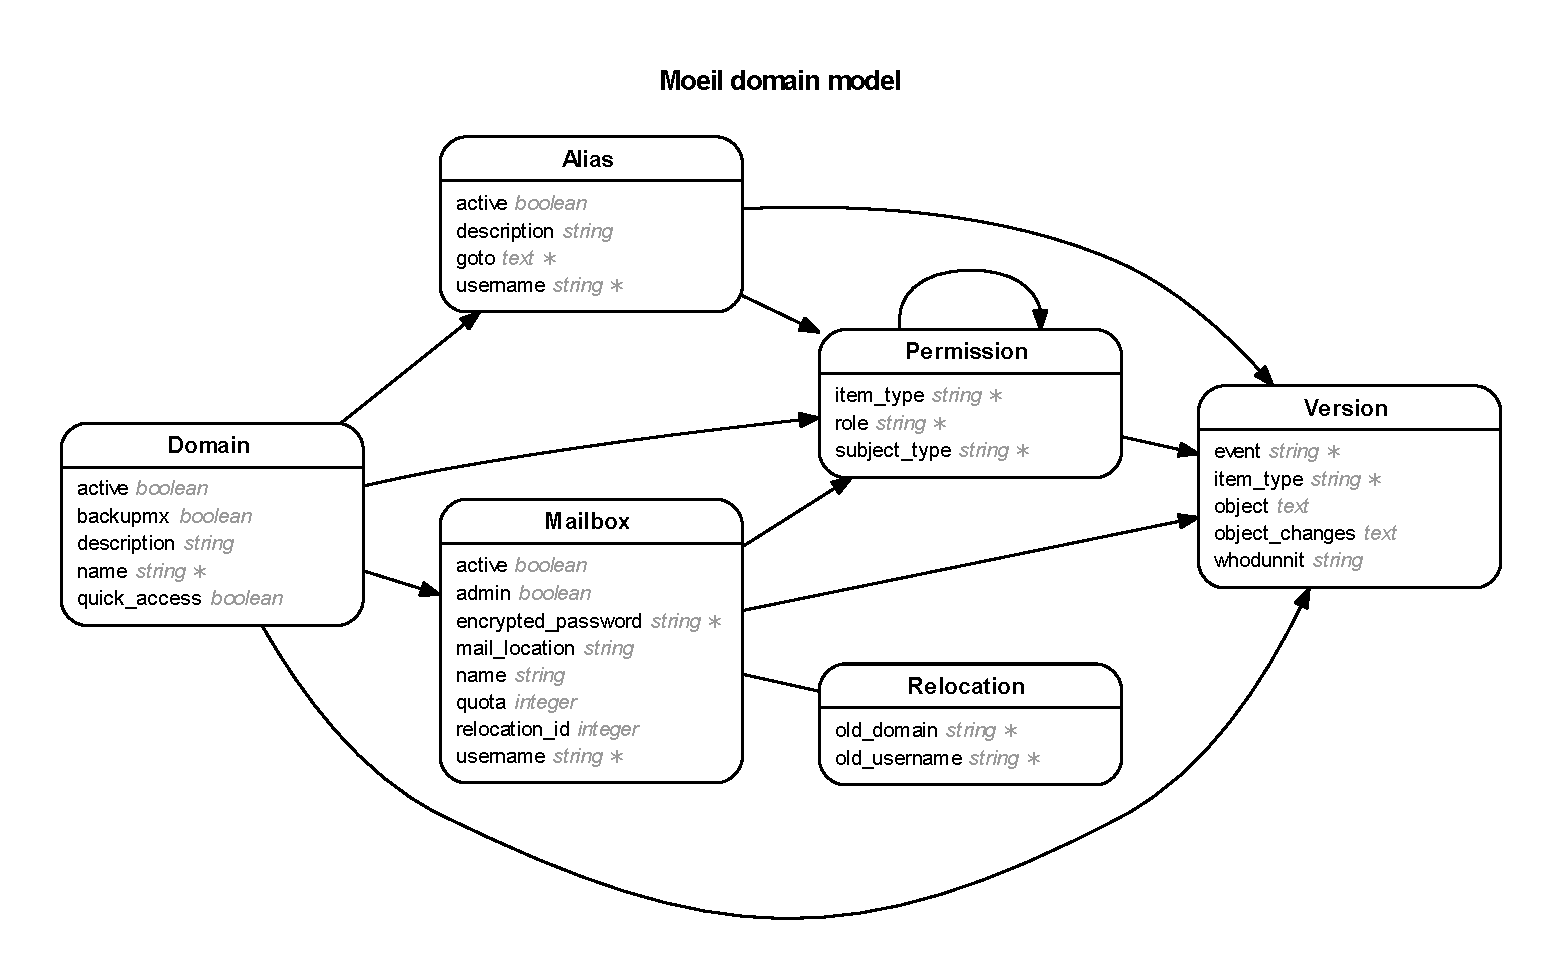
\includegraphics[width=\textwidth]{images/erd.pdf}

			\noindent
			The model classes will be examined individually in the following
			subsections. In this chapter, whenever a resource type is
			mentioned, which corresponds to an actual \ac{Rails} model class,
			it is written in a monospace font and -- as the class name --
			capitalized, like \texttt{Mailbox}. Attributes of models are also
			in monospace font, but lowercase, as the \texttt{username}
			attribute of a \texttt{Mailbox} for example.

			\subsubsection{Domains}
				For \texttt{Domains} the following attributes are saved per
				record: \texttt{name} (which is the actual domain- or hostname,
				\texttt{description}, \texttt{backupmx} (indicates, if the
				domain is specified as backup MX), \texttt{active},
				\texttt{quick\_access} (indicates, if the domain edit is
				reachable through a quick access menu in the \ac{UI}),
				\texttt{mx\_set} (for automatically saving, if the MX record in
				the DNS points to the correct mail server) and the timestamps
				of creation and last update. \texttt{Domains} are connected to
				many \texttt{Mailboxes} and \texttt{Aliases} to reflect the
				affiliation of the latter.

			\subsubsection{Mailboxes}
				A \texttt{Mailbox} is connected to its \texttt{Domain} and
				possibly also to one \texttt{Relocation} and has the attributes
				\texttt{username} (which is the part in front of the
				domain in the E-Mail address), \texttt{encrypted\_password}
				(containing the password hash), \texttt{name} (for a given name
				for example), \texttt{mail\_location} (which is empty by
				default but can be used to move the users mail data location),
				\texttt{quota}, \texttt{active}, \texttt{admin} and timestamp
				attributes for saving the date of creation or the last update.
				As a password hashing algorithm, currently only
				\texttt{sha512-crypt} is supported.

			\subsubsection{Aliases}
				\texttt{Aliases} represent mail forwardings and are also
				connected to their affiliated \texttt{Domain}. They have the
				attributes \texttt{username}, \texttt{goto} (which is the
				target of the forwarding and can contain one or more internal
				or external E-Mail addresses seperated by commas),
				\texttt{active}, \texttt{description} and timestamps of
				creation and last update.

			\subsubsection{Permissions}
				\texttt{Mailbox} records (or users) are also used for the login
				to \emph{Møil}. There are administrators and regular users.
				Administrators are allowed to edit any resources. Through a
				\texttt{Permission}, a \texttt{Mailbox} (the \texttt{subject})
				can be given access to \texttt{Domains} (the \texttt{item}).
				The rights on these \texttt{Domains} depend on the
				\texttt{role} of the user in this context. With an owner
				\texttt{role}, users can manage any aspect of the
				\texttt{Domains}. The editor \texttt{role} allows users to
				manage \texttt{Mailboxes} and \texttt{Aliases} of that.
				\texttt{Domain}. The \texttt{Permission} model is implemented
				polymorphic. Its \texttt{subject} and \texttt{item} attributes
				are not bound to \texttt{Mailboxes} and \texttt{Domains} (as in
				the current implementation). It is possible to extend the
				implementation easily to allow even more fine-grained
				permissions (for certain \texttt{Mailboxes} for example).

			\subsubsection{Versions}
				As seen in the graph, \texttt{Domains}, \texttt{Mailboxes},
				\texttt{Aliases} and \texttt{Permissions} are versioned, which
				means that changes to resources of any of these types are
				tracked in the audit log and are revertable for administrators.
				On any change, a reference to the corresponding resource
				(\texttt{item\_id} and \texttt{item\_type}), the type of change
				(\texttt{event}), the transacting individual
				(\texttt{whodunnit}), the serialized \texttt{object} (only on
				deletions, can be used for undo), the \texttt{object\_changes}
				(only on updates) and the point in time (\texttt{created\_at})
				are saved.

			\subsubsection{Relocations}
			\label{sec:moeil:model:relocation}
				The relocation model is in fact updated but actually not
				further used, currently. Whenever a \texttt{Domain} or
				\texttt{Mailbox} is renamed, it is necessary to move the
				corresponding folders in the file system of the Mail Store.
				These moves are represented as \texttt{Relocation} resources
				saving \texttt{old\_domain} and \texttt{old\_username} values,
				which can be read by a daemon (yet to be implemented) running
				on the actual Mail Store.

		\subsection{Perspective}
			Not least through the evaluation of the different solutions for
			Open Source mail system administration user interfaces, some
			possible features for Møil become obvious.

			\begin{description}
				\item[\rm Better \ac{CLI}]\ \\
					Currently, Møil has seperate \ac{CLI} tools for the most
					important tasks like managing domains and mailboxes and
					importing data from an \emph{postfix.admin} installation.
					This can be expanded into a single \ac{CLI} utility with
					better support for the features, the web user interface
					offers.

				\item[\rm Spam and virus check integration]\ \\
					Some compared solutions integrate \texttt{amavisd-new} by
					shared database tables. After this being clear, there is
					not much left to be solved conceptually for a spam and
					virus check integration and this becomes a question of time.

				\item[\rm Support for server-side filters]\ \\
					The support for server-side filters in Møil was already
					examined and begun but at first, a Ruby library for the
					ManageSieve protocol has to be implemented, because the
					only one existing is not maintained anymore and became
					disfunctional.
			\end{description}

		\subsection{Setup}
			Installation instructions and configuration files will not appear
			itself in this section. Instead, they will be linked to. This
			should make this document a little more long-lasting, because setup
			instructions usually are subject to frequent changes.

			\subsubsection{Relevant configs for \emph{postfix} and \emph{dovecot}}
				The relevant configuration files for \emph{postfix} and
				\emph{dovecot} (especially regarding to the \ac{SQL} statements
				compatible to \emph{Møil}) can be found in the source code
				repository on GitHub in the folders \texttt{doc/postfix} and
				\texttt{doc/dovecot}\footnote{\url{https://github.com/nning/moeil/tree/master/doc}}.

			\subsubsection{Setup of the rails application}
				The setup of the rails app for testing or deployment on
				OpenShift is described in the main
				README\footnote{\url{https://github.com/nning/moeil}} file of
				\emph{Møil}. A deployment in web servers like \emph{Apache},
				\emph{nginx} and \emph{lighttpd} is made similar to any other
				current \ac{Rails} project. (Also it is possible to deploy with
				\emph{capistrano}.) More detailed and beginner-friendly
				instructions will be provided in the main README file at a
				later point.

	\appendix

	\newpage
	\section{Numbered index of criteria}
	\label{sec:appendix:criteria}
		\begin{easylist}
			& Data model
			&& Normalized schema
			&& \emph{postfix.admin} compatible
			&& \emph{postfix.admin} import
			&& Schema migrations
			&& Systematic database independence
			\s

			& Features
			&& Basic domain, mailbox and alias management
			&& Password changing for users
			&& Access control
			&& Others
			&&& Audit trail
			&&& Vacation
			&&& Sieve
			&&& Spam front-end
			\s

			& Security \& robustness
			&& Password hashing
			&& Test coverage
			&& Containability
			\s

			& Responsive design
			&& Mobile devices
			&& \ac{CLI} support
		\end{easylist}

	\newpage
\section*{Acronyms}
\begin{acronym}
	\acro{CLI} {Command line interface}
	\acro{CRUD}{Create, read, update and delete}
	\acro{DBMS}{Database Management System}
	\acro{SMTP}{Simple Mail Transfer Protocol}
	\acro{SQL} {Structured Query Language}
\end{acronym}


	\printbibliography

\end{document}
